\documentclass[tikz,border=5mm,12pt]{standalone}
\usetikzlibrary{positioning,backgrounds}

\newcommand\sep{10mm}
\newcommand\scopesep{40mm}
\newcommand\drawpeople{
  \path (0,0) coordinate (P1)
    -- ++(360-22.5:\sep) coordinate (P2)
    -- ++(360-22.5-45:\sep) coordinate (P3)
    -- ++(360-22.5-90:\sep) coordinate (P4)
    -- ++(360-22.5-135:\sep) coordinate (P5)
    -- ++(360-22.5-180:\sep) coordinate (P6)
    -- ++(360-22.5-180-45:\sep) coordinate (P7)
    -- ++(360-22.5-180-90:\sep) coordinate (P8);

  \node[person] at (P1) {1};
  \node[person] at (P2) {2};
  \node[person] at (P3) {3};
  \node[person] at (P4) {4};
  \node[person] at (P5) {5};
  \node[person] at (P6) {6};
  \node[person] at (P7) {7};
  \node[person] at (P8) {8};
}
\begin{document}
  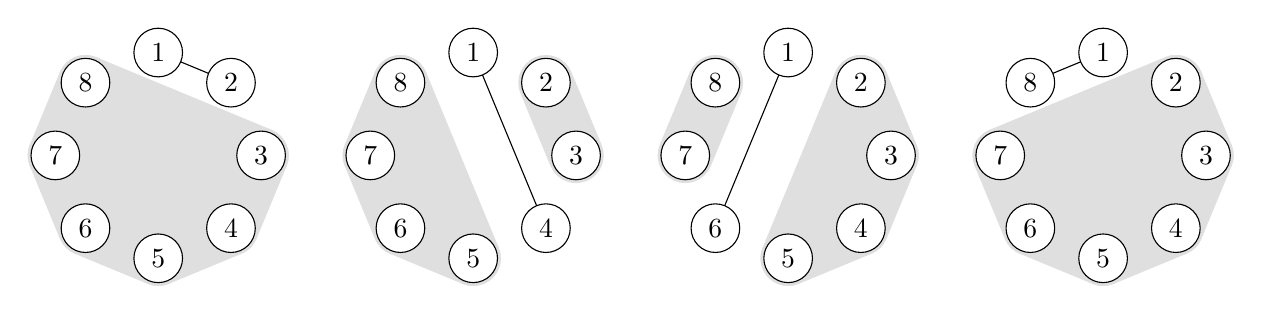
\begin{tikzpicture}[
    person/.style={draw,circle,fill=white},
    shadecolor/.style={lightgray!50},
    shade/.style={shadecolor,line width=20pt,line cap=round}
  ]
    \begin{scope}
      \drawpeople

      % line and shade
      \begin{scope}[on background layer]
        \draw (P1) -- (P2);

        \draw[shade] (P3) -- (P4); % hack to avoid non-rounding corners
        \draw[shade] (P4) -- (P5);
        \draw[shade] (P5) -- (P6);
        \draw[shade] (P6) -- (P7);
        \draw[shade] (P7) -- (P8);
        \draw[shade] (P8) -- (P3);
        \draw[fill,shadecolor] (P3) -- (P4) -- (P5) -- (P6) -- (P7) -- (P8) -- cycle;
      \end{scope}
    \end{scope}

    \begin{scope}[xshift=\scopesep]
      \drawpeople

      % line and shade
      \begin{scope}[on background layer]
        \draw (P1) -- (P4);

        \draw[shade] (P5) -- (P6);
        \draw[shade] (P6) -- (P7);
        \draw[shade] (P7) -- (P8);
        \draw[shade] (P8) -- (P5);
        \draw[fill,shadecolor] (P5) -- (P6) -- (P7) -- (P8) -- cycle;

        \draw[shade] (P2) -- (P3);
      \end{scope}
    \end{scope}

    \begin{scope}[xshift=2*\scopesep]
      \drawpeople

      % line and shade
      \begin{scope}[on background layer]
        \draw (P1) -- (P6);

        \draw[shade] (P2) -- (P3);
        \draw[shade] (P3) -- (P4);
        \draw[shade] (P4) -- (P5);
        \draw[shade] (P5) -- (P2);
        \draw[fill,shadecolor] (P2) -- (P3) -- (P4) -- (P5) -- cycle;

        \draw[shade] (P7) -- (P8);
      \end{scope}
    \end{scope}

    \begin{scope}[xshift=3*\scopesep]
      \drawpeople

      % line and shade
      \begin{scope}[on background layer]
        \draw (P1) -- (P8);

        \draw[shade] (P2) -- (P3);
        \draw[shade] (P3) -- (P4);
        \draw[shade] (P4) -- (P5);
        \draw[shade] (P5) -- (P6);
        \draw[shade] (P6) -- (P7);
        \draw[shade] (P7) -- (P2);
        \draw[fill,shadecolor] (P2) -- (P3) -- (P4) -- (P5) -- (P6) -- (P7) -- cycle;
      \end{scope}
    \end{scope}
  \end{tikzpicture}
\end{document}
